\section{Problem Statement}

Maintenant que nous sommes bien outillés,  nous allons pouvoir décrire notre problème,  c'est-à-dire notre question de base que nous résoudrons par la suite.  Ce chapitre s'attarde donc à décrire les éléments du problème tels qu'ils ont été présentés au début ou pendant la réalisation de ce mémoire.  Tout d'abord,  nous allons décrire le cas de l'organisation BuurtPensioen et ses besoins,  qui furent le point de départ du mémoire.  Ensuite,  nous décrirons le logiciel créé par un groupe d'étudiants du cours LSINF/INFO2255 qui a été présentée en décembre et qui a servi de base pour être transformé et devenir le framework final.

\subsection{BuurtPensioen}

BuurtPensioen \cite{buurtpensioen} (\"pens('i)ons voisin\",  en français) est un projet néerlandophone basée à Bruxelles issue de la collaboration entre diverses associations de la capitale.  Ce projet regroupe une communauté de membres qui s'entraident mutuellement.  Le principe est le suivant.  Dans la vie,  nous sommes assez autonomes pendant l'âge adulte mais cela diminue avec l'âge.  Ainsi,  les personnes plus âgées deviennent dépendant de l'aide d'autres personnes.  C'est dans ce sens que le système de pensions a été créé : on épargne de l'argent lorsqu'on est en âge de travailler et on le reçoit en retour une fois que l'on prend sa retraite.  L'organisation BuurtPensioen est basée sur ce principe mais ne fonctionne pas avec de l'argent mais plutôt avec du temps.  En effet,  lorsque quelqu'un rend un service à une autre personne,  on compte en minutes ou en heures,  le temps que ce service a pris.  La personne qui a aidé "reçoit" alors ce temps et peut le cumuler.  Avec en perspective d'avoir une certaine réserve de temps pour le moment ou cette personne ne sera plus en capacité de se débrouiller seule.  Elle pourra alors utiliser son "capital-temps" afin de se faire aider.

Ce système a été mis en place suite à un constat que les aides organisées par l'état pour les personnes âges sont de moins en moins présentes en Belgique et,  au delà de ce constat financier,  beaucoup de ces mêmes personnes sont également isolées du reste du monde.  La solution proposée par BuurtPensioen permet d'aider la personne âgée mais cette aide est aussi une occaison de reconnecter la personne avec le reste de la société.   

Un projet pilote a été lancé en novembre 2013 dans la commune de Neder-over-Heembeek.  Celui-ci a remporté un vif succès et il est envisagé de créer d'autres projets dans ou aux alentours de Bruxelles.  

Cependant,  le projet BuurtPensioen aimerait d'abord se munir d'un outil plus automatisé avant d'élargir son terrain d'action.  Pour cela,  une collaboration avec l'UCL a été mise en place en 2014.  Le professeur Kim Mens,  enseignant du cours "SINFINFO 2255 Projet de développement logiciel",  a participé à l'élaboration d'un cahier de charges pour la création de cette plateforme ( voir Annexe 1 \ref{bpse} ).  L'objectif étant de proposer ce sujet comme projet pour le cours pré-cité.  
\newline
\newline
Pour se faire une petite idée du style d'outil qui a été demandé par le consortium Buurtpensioen,  nous allons parcourir rapidement quelques éléments clés de ce cahier des charges.

\begin{description}

\item [Membres]
Le logiciel créé doit gérer un système de membres de différent types.  D'abord,  les membres "normaux".  Il s'agit des utilisateurs finaux de l'application,  c'est-à-dire les personnes âgées ainsi que celles qui les aident.  Ensuite,  des membres du type "administratif",  c'est-à-dire des gestionnaires du projet BuurtPensioen.  Ces gestionnaires peuvent être de 2 niveaux : soit administrateurs d'une région géographique (branches),  soit administrateurs du système dans son entièreté.

\item [Crédits]
Chaque membre doit posséder son propre "compte" de temps accumulé.  Celui-ci représente la pension du membre,  c'est-à-dire la somme des services qu'il a déjà rendu,  valorisés en unité de temps,  et qui pourra être utilisé en cas de besoin dans l'avenir.  De plus,  un système de dons doit être mis en place afin de permettre à des membres d'offrir une partie ou l'entièreté de son crédit à une autre personne.

\item [Branches]
La solution proposée doit inclure un système de "branches".  Cette appellation désigne des antennes locales de l'organisation,  que les membres pourraient rejoindre.  Les antennes locales (= branches) représentent des zones géographiques.  
Chaque branche possède,  dans le système,  des informations qui lui sont propres telles que son adresse,  le nom de l'administrateur de cette branche,  etc.

\item [Offres-Demandes]
Le système aura bien sur pour but de mettre les membres en relation sur base des offres et demandes qu'ils encoderont.  Ainsi,  les personnes dans le besoin seront invitées à encoder leurs demandes dans le système en fournissant les informations nécéssaires pour le service demandé,  c'est-à-dire le moment où le sevice est demandé,  le type de service,  le temps que cela prendrait, etc.

\item [Divers]
Diverses exigences sont également à prendre en compte et concernent l'application dans son entièreté.  Premièrement,  étant donné que le système sera utilisé par des personnes pouvant ne pas être habituées à l'informatique,  il faut que l'application soit facile d'utilisation notamment via une interface simple.  Ensuite,  la solution proposée doit prendre en compte les aspects de sécurité afin que les données encodées par les membres ne soient pas dérobées ou altérées.  Enfin,  il est demandé de mettre en place un système de statistiques à propos des membres ainsi que de l'utilisation (nombre d'offres/demandes,  temps de réponse à une demande, \dots ) et d'autres fonctionnalités de plus petite utilité tels qu'une possibilité de lien avec Facebook,  l'utilisation de Google Maps, \dots .

\item [Statistiques pour la VUB]
Lors d'une rencontre avec Liesbeth De Donder,  doctorante à la VUB,  nous avons également abordé le thème des statistiques qui devraient être accessibles dans l'application.  En effet,  l'université de Bruxelles aimerait avoir la possibilité de récolter et traiter des données concernant l'utilisation et les utilisateurs des systèmes tels que celui qui doit être développé pour Buurtpensioen.  Au départ,  les statistiques ne sont que l'une des fonctionnalités demandées pour Het Buurtpensioen.  Mais sachant que des acteurs extérieurs sont intéressés par les statistiques,  nous pouvons considérer que les statistiques sont un point important de l'application.  Du moins,  pour le framework développé puisque cet "appui" concernant les statistiques ne fait pas partie du cahier des charges initialement donné comme référence de base aux étudiants du cours de Software Development Project.   

\end{description}

Pendant tout le premier quadrimestre,  les étudiants du cours ont donc travaillé à l'élaboration d'une solution répondant à ce cahier des charges.  Le travail étant réalisé par groupes de 6 à 8 étudiants,  il a résulté de ce cours plusieurs propositions de solutions.  Parmi celles-ci,  la solution du Groupe 8 a été celle qui a le plus retenu l'attention de Katleen Deruyter,  personne de contact de BuurtPensioen pour tout le processus de collaboration entre l'UCL et l'organisation.  Cette solution a été analysée et utilisée pour la deuxième partie du mémoire (réalisation du framework).  C'est pourquoi nous allons maintenant décrire rapidement la solution proposée.


\subsection{Solution proposée dans le cadre du cours LSINF/INFO 2255}

La solution proposée par le Groupe 8 du cours LSINFINFO2255 de 2014-2015 consiste en un site web utilisant Django (voir section \ref{django}).  Nous allons parcourir rapidement l'application développée afin de mieux se rendre compte du genre d'outil désiré.

Commençons par la page d'accueil du site internet.  

\vspace{1cm}
\fbox{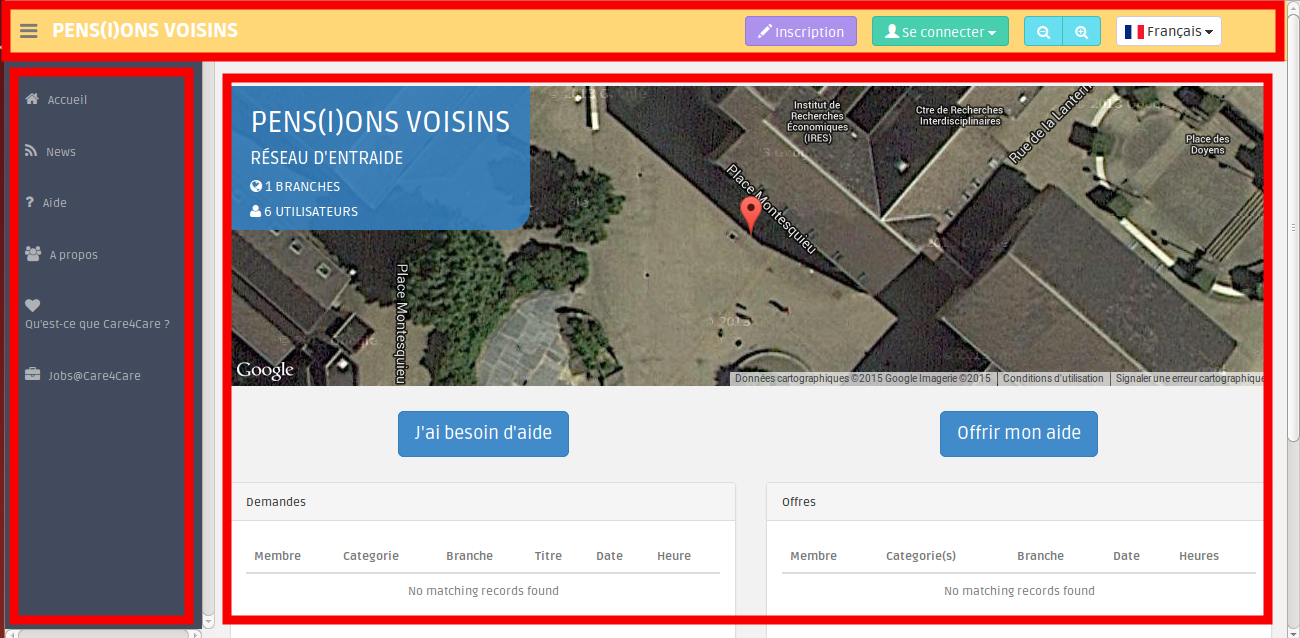
\includegraphics[scale=0.30]{gr8home1.png}}
\vspace{1cm}

On observe (en rouge) 3 zones principales sur l'écran : le menu de navigation sur la gauche,  le menu de connexion dans la barre supérieure et la zone de contenu sur le reste de la page.  
Tout d'abord,  le menu de connexion dans le haut de la page permet à l'utilisateur de s'enregistrer ou de s'identifier s'il est déjà inscrit.  On peut également changer la langue du site internet.  Notons que toutes les langues ne sont pas encore implémentées à 100\%.  
Ensuite,  le menu à gauche peut varier selon qu'on est connecté ou non.  Il permet de naviguer entre les différentes pages principales du site.  
Enfin,  la partie contenu du site affiche,  à l'accueil,  une carte Google Maps reprenant les branches existantes localisées par une pipette rouge,  et juste en dessous,  deux tableaux reprenant chacun la liste des offres et la liste des demandes qui ne sont pas encore complétées.  

Si on suit un scénario classique sur le site,  on peut commencer par se rendre sur la page d'inscription au site afin de voir à quoi celle-ci ressemble.

\vspace{1cm}
\fbox{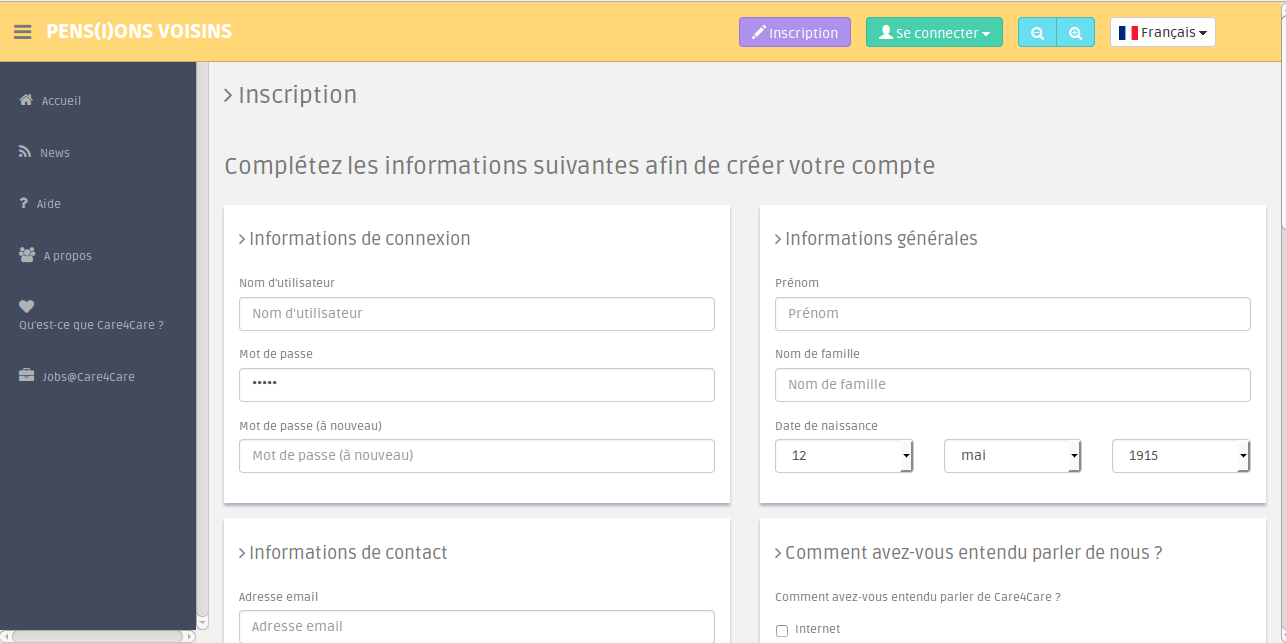
\includegraphics[scale=0.30]{gr8inscr.png}}
\vspace{1cm}

Sur cette page,  on accède au formulaire d'inscription demandant de renseigner des données d'identification habituelles telles que nom d'utilisateur et mot de passe,  adresse email et autres mais il est également demandé de choisir une branche (= une antenne locale du projet) que l'on rejoindra dès le début.  

Après s'être enregistré puis connecté,  nous pouvons retrouver nos informations sur la page Profil.

\vspace{1cm}
\fbox{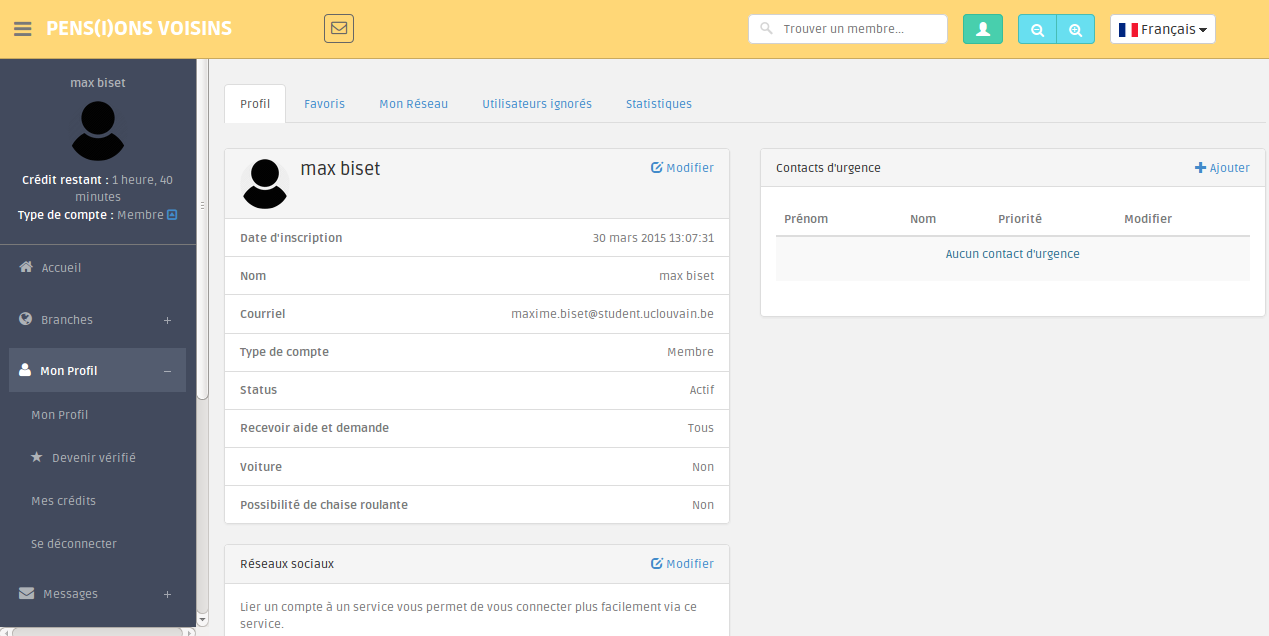
\includegraphics[scale=0.30]{gr8profil.png}}
\vspace{1cm}

Ici,  on retrouve les informations encodées lors de l'inscription mais aussi un accès à d'autres données modifiables telles que les listes d'utilisateurs favoris ou ignorés ainsi que l'accès au statistiques du compte.

Il nous reste maintenant à attaquer le fond même du site,  c'est à dire les échanges.  Pour cela,  nous pouvons analyser de plus près la page d'accueil.  

\vspace{1cm}
\fbox{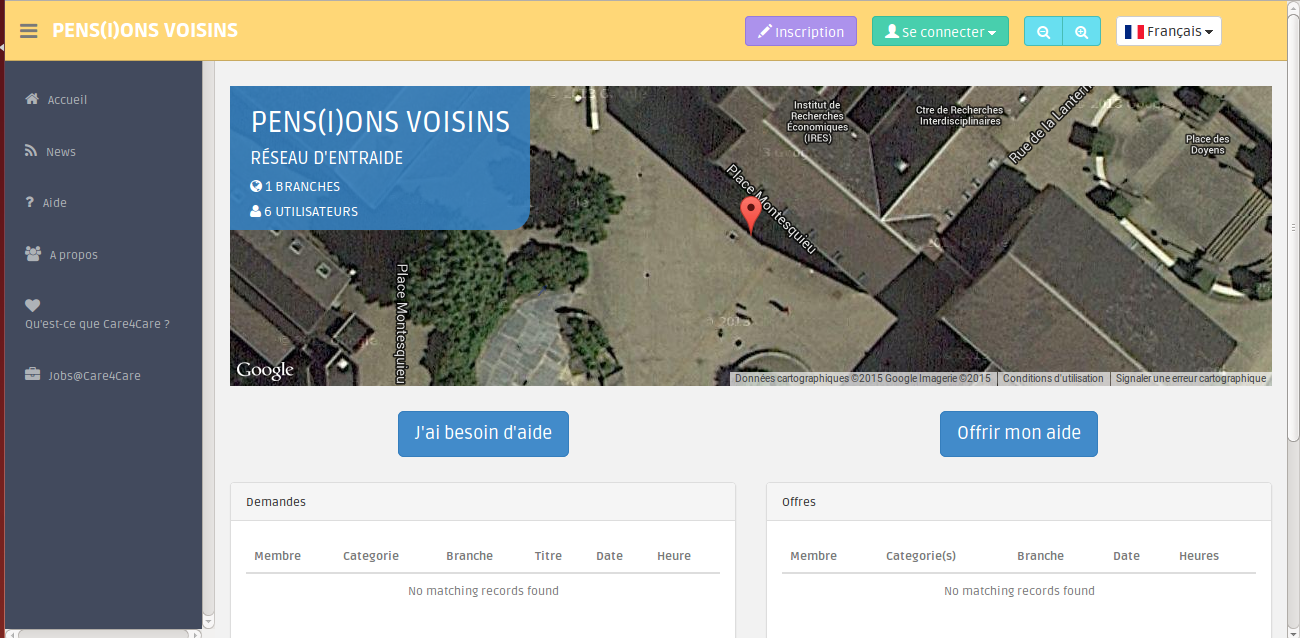
\includegraphics[scale=0.30]{gr8home.png}}
\vspace{1cm}

On remarque sur cette page que 2 catégories existent sur le site : les offres d'aide et les demandes d'aide.  Celles-ci apparaissent dans deux parties de l'écran.  Un simple bouton permet également d'enregistrer une demande ou une offre.  

Nous allons maintenant voir un aperçu d'une page destinée à encoder une demande d'aide.

\vspace{1cm}
\fbox{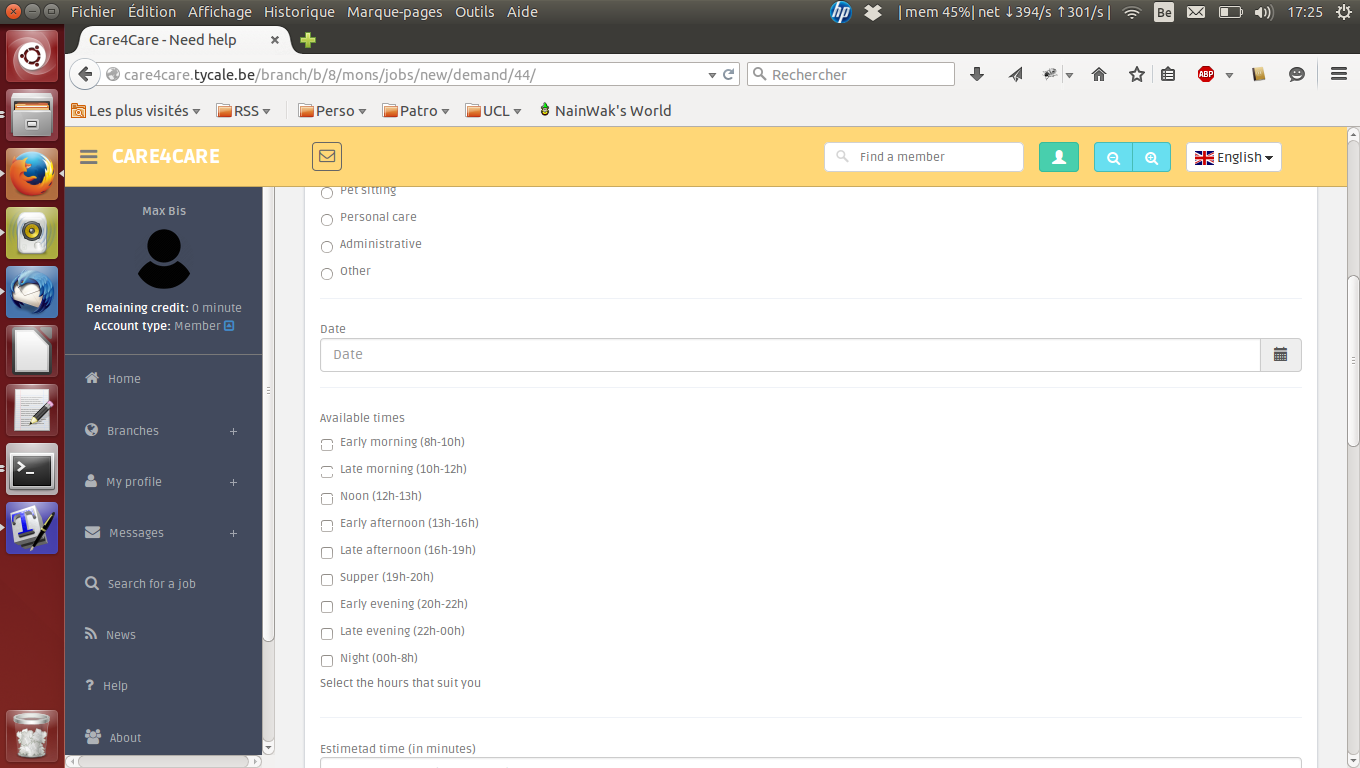
\includegraphics[scale=0.30]{encoder.png}}
\vspace{1cm}

Sur cette page,  l'utilisateur est invité à encoder les informations liées aux service recherché.  Pour cela,  il peut choisir un type de service,  le moment où celui-ci doit avoir lieu ainsi que le lieu.  Il est également possible d'entrer un titre et une description du service.  Après que la demande de service soit encodée dans le système,  elle apparait dans la liste des demandes non remplies.  Lorsqu'un utilisateur répond à la demande,  l'initiateur de celle-ci est averti et peut valider la réponse.  Une fois le service rendu,  la demande n'est plus affichée dans la liste.

Nous avons ainsi pu faire un rapide tour de l'application créée par les étudiants du cours de Software Development Project.

\subsection{Autres organisations existantes}
\phantomsection
\label{autresOrgas}
Après avoir observé ce cas principal de BuurtPensioen,  nous allons aborder rapidement quelques autres organisation et outils existants.  Ceci permet de se rendre compte du paysage des applications possibles pour un framework tel que nous voulons le développer.  Dans le domaine des échanges locaux,  ces informations ont été récoltées selon 2 cannaux : d'une part,  une réunion avec divers représentants d'organisations semblables à BuurtPensioen qui a eu lieu en octobre 2014 et d'autre part,  diverses recherches sur internet.

\begin{description}

\item [Cyclos (http://www.cyclos.org/)]

Cyclos est un logiciel d'online et mobile banking.  Il ne s'agit,  ici,  que d'un outil qui peut être utilisé par des organisations.  Cet outil est adaptable à plusieurs situations et permet d'utiliser diverses monnaies dont des monnaies complémentaires.  Il est développé par le réseau Social TRade Organisation (\cite{STRO}) et plusieurs versions existent : une gratuite et open-source téléchargeable sur le site web de Cyclos,  un système de services Cyclos pour les communautés locales (il est possible de créer son initiative locale via le site officiel de Cyclos),  et enfin une version "pro" destinée aux grandes organisations avec des prix variant de 1000 à 3000 euros de frais d'abonnement par an,  voire plus selon négociation lorsque les organisations sont de très grande taille.  
Enfin,  l'outil Cyclos est sous licence GNU General Public Licence.

\item [System d'Entraide Local (SEL) (www.sel-lets.be/ )]

Le SEL est en même temps un outil et des organisations.  Ce site propose aux communautés de s'inscrire chez eux et de leur fournir les services d'un outil permettant l'échange de services.  Ces derniers sont catégorisés dans diverses thématiques.  Chaque communauté possède son minisite sur lequel les utilisateurs peuvent s'enregistrer pour encoder leurs offres et demandes de services.  Les services vont du ménage au bricolage en passant par l'éducation et l'apprentissage.  

\item [QOIN (http://www.qoin.org)]
\phantomsection
\label{QOIN}

QOIN est une entreprise de services de management et d'informatique destiné à la mise en place de communautés locales de monnaies alternatives.  Dans ce cadre,  cette organisation a développé 2 logiciels qui sont utilisés dans la région d'Amsterdam.  Le premier logiciel,  TradeQoin,  est destiné aux petites et moyennes entreprises qui se rendent des services entre elles.  Le second,  ShareQoin,  est utilisé par 10 monnaies alternatives différentes et est destiné à des personnes physiques.  

\item [Troeven.be (https://www.troeven.be/)]
Troeven est un projet en phase de test mené dans la commune de Turnhout (province d'Anvers) et qui utilise l'outil TradeQoin (défini juste avant).  Ce projet utilise comme monnaie des "troeven" ("atouts" en français) et n'est disponible qu'en néérlandais.

\end{description}

Nous avons listé ici quelques outils et organisations qui ont servi de sources d'informations pour ce mémoire.  L'objectif a été d'avoir un aperçu de ce qui existe au niveau des outils pour gérer des projets du même genre que Buurtpensioen ainsi que d'autres projets existants.  

Étant donné que nous allons développer un framework,  la question se pose de savoir quel sera le logiciel d'origine qui va être utilisé comme base pour le développement de ce framework opensource qui pourrait être appliqué,  par exemple,  au cas du projet Buurtpensioen.  Notons que,  dans la pratique,  cette question s'est posée après l'analyse du domaine pour des raisons de timing mais il semble opportun de répondre à cette question ici,  après avoir détaillé les systèmes existants.  
Pour répondre à la demande d'un framework,  2 propositions ont été envisagées pour servir de base : l'outil Cyclos ou celui développé par le groupe d'étudiants et destiné à Buurtpensioen.   En effet,  ces 2 logiciels sont open source et peuvent donc être ré-utilisés.  L'avantage de Cyclos est qu'il possède de nombreuses fonctionnalités (mais pas toutes aceessibles dans la version téléchargeable).  Le second outil,  quant à lui,  a été choisi parmi plusieurs solutions comme étant celle qui répondait le mieux aux demandes de Burrtpensioen,  une des utilisations finales possibles du framework.  C'est d'ailleurs cet argument là qui va faire pencher notre choix car Cyclos est un logiciel à paramétrer tandis que la solution des étudiants est un logiciel fonctionnel prêt à l'emploi.  Cela permet d'économiser une étape supplémentaire pour le développement du framework.  Le choix est donc fait de partir de la solution développée par le groupe d'étudiants pour développer un framework plus global.

Ceci clôture le chapitre sur l'explication du problème à résoudre.  La prochaine étape consiste à analyser de plus près le domaine dans lequel nous allons devoir développer notre framework.  


